% Provenance (never printed): see sources/outline_sources.md (Year 2: anatexis, migmatites,
% granite types and their sources). Wet granite solidus from Stern and Wyllie (1981) and
% Boettcher and Wyllie (1968); dehydration-melting brackets from Patino Douce and Harris
% (1998), Berger and Kalt (1999), Skjerlie and Johnston (1996); water solubility from Holtz
% et al. (1995); migmatite terms from the IUGS-SCMR proposal and BGS RR 99-02; aluminosity
% after Shand (as given by Moyen et al. 2017); figure data in figdata/bachelor-2/anatexis.py
% (paths from ptpaths.py); exercise and problem values in the Book 4 scratch calculator
% calc/ch12.py.
\chapter{La fusión de la corteza: migmatitas y granitos}\label{ch:b2:crustal-melting}

El granito es lo que hace ligeros a los continentes, y el manto no puede formarlo directamente: los
fundidos de la \omterm{def:b2:mantle-melting:peridotites}{peridotita} son basaltos. La mayor parte del granito es la corteza continental fundiéndose a sí misma.
Cuando la raíz engrosada de una cordillera se calienta, cuando el basalto se estanca bajo la corteza, o cuando una
roca caliente sube y su presión baja, las micas y los anfíboles de la corteza profunda ceden
su agua, aparece un líquido granítico entre los granos, y la roca se convierte en una
\omterm{def:b2:crustal-melting:migmatite}{migmatita}, mitad metamórfica, mitad ígnea. Este capítulo sigue a ese líquido desde sus primeras
películas hasta el \omterm{def:b2:magma-emplacement:bodies}{plutón} que puede construir, y lee en la química de un granito la roca de la que
procede.

\begin{recall}
\textbf{Del volumen de bachillerato}: el granito, el granitoide y la granodiorita; las rocas félsicas y máficas;
las raíces de las cordilleras. \textbf{Del volumen de primer año}: la producción de calor
radiogénico en la corteza; la hidrólisis de los silicatos y los minerales de la arcilla. \textbf{De los libros de química}: el solidus y el liquidus
de un sistema binario, la masa molar y la cantidad de sustancia. \textbf{Del
\cref{ch:b2:magma-emplacement}}: los \omterm{def:b2:magma-emplacement:bodies}{diques}, los plutones y los \omterm{def:b2:magma-emplacement:ascent}{diapiros}. \textbf{Del
\cref{ch:b2:mantle-melting}}: la \omterm{def:b2:mantle-melting:melting}{fusión parcial}, la \omterm{def:b2:mantle-melting:peritectic}{fusión incongruente} y la \omterm{def:b2:mantle-melting:melting}{fusión por
descompresión}. \textbf{Del \cref{ch:b2:metamorphic-facies}}: las \omterm{def:b2:metamorphic-facies:protoliths}{metapelitas}, la \omterm{def:b2:metamorphic-facies:clapeyron}{pendiente de Clapeyron} de
una reacción y las facies. \textbf{Del \cref{ch:b2:pt-paths}}: las \omterm{def:b2:pt-paths:ptt}{trayectorias P--T--t} y el
modelo de engrosamiento de la corteza.
\end{recall}

\section{Por qué se funde la corteza}\label{sec:b2:crustal-melting:why}

La palabra que lo designa es antigua y sencilla.

\begin{definition}[Anatexia]\label{def:b2:crustal-melting:anatexis}
La \emph{anatexia}\index{anatexia} es la fusión de una roca, cualquiera que sea el grado de fusión;
en la práctica la palabra se usa para la \omterm{def:b2:mantle-melting:melting}{fusión parcial} de la corteza continental.
\end{definition}
% ledger: scmr:migmatite

\subsection*{El solidus húmedo}

El granito solo funde a baja temperatura cuando está húmedo. Stern y Wyllie fundieron un granito de
biotita del \omterm{def:b2:magma-emplacement:bodies}{batolito} de Sierra Nevada con exceso de agua: el primer líquido apareció a
\qty{680}{\celsius} a \qty{2}{kbar} y a \qty{620}{\celsius} a \qty{10}{kbar}, y la
roca entera solo estaba fundida \qty{35}{\celsius} por encima del solidus a \qty{2}{kbar}, pero
\qty{105}{\celsius} por encima a \qty{10}{kbar}. El mismo granito, estudiado antes por
Boettcher y Wyllie, empezaba a fundir a \qty{605}{\celsius} a \qty{15.3}{kbar}; cerca de
\qty{17}{kbar} su plagioclasa se descomponía en jadeíta y cuarzo, y a partir de ahí el solidus
volvía a subir, hasta alcanzar \qty{670}{\celsius} a \qty{27}{kbar}.
% ledger: sw81:wet-solidus, bw68:wet-solidus

El solidus húmedo baja al aumentar la presión, al contrario que un solidus seco. La razón está en adónde
va el agua. El agua libre es un fluido de baja densidad; disuelta en el fundido ocupa muy
poco espacio: Holtz y colaboradores hallaron que su volumen molar parcial en un fundido granítico está cerca
de \qtyrange{10}{12}{\cubic\centi\metre\per\mole}, frente a \qty{18}{\cubic\centi\metre\per\mole}
del agua líquida en condiciones ambientales y más aún para un fluido caliente. La reacción de fusión
\[\text{cuarzo} + \text{feldespatos} + \ce{H2O}\ (\text{fluido}) \longrightarrow
\text{fundido hidratado}\]
tiene por tanto una variación de volumen negativa, mientras que su variación de entropía, como en toda fusión, es
positiva: por la relación de Clapeyron del \cref{ch:b2:metamorphic-facies}, su pendiente
$\mathrm{d}P/\mathrm{d}T = \Delta S/\Delta V$ es negativa. La presión deja además entrar más agua
en el fundido: para un fundido haplogranítico a \qty{800}{\celsius} el contenido de saturación sube
de un \qty{2.80}{\percent} en masa a \qty{0.5}{kbar} a un \qty{9.97}{\percent} a
\qty{5}{kbar} y un \qty{13.82}{\percent} a \qty{8}{kbar}, cerca de un \qty{1.27}{\percent} más
por kilobar entre 3 y \qty{8}{kbar}.
% ledger: holtz95:solubility

\begin{omfigure}
\centering
\begin{tikzpicture}
\begin{axis}[omrecord, width=0.5\linewidth, height=4.8cm,
  xmin=0, xmax=9, ymin=0, ymax=15, xlabel={$P$ (\unit{kbar})},
  ylabel={\ce{H2O} en el fundido (\unit{\percent})},
  tick label style={font=\scriptsize}, label style={font=\small}]
\addplot[only marks, mark=*, mark size=1.6pt, blue!70!black]
  table[x=P_kbar, y=H2O_wt] {figdata/out/bachelor-2-anatexis-water.dat};
\addplot[thick, red!75!black] table[x=P_kbar, y=H2O_wt] {figdata/out/bachelor-2-anatexis-waterfit.dat};
\end{axis}
\end{tikzpicture}
\par\smallskip{\small Agua que puede disolver un fundido haplogranítico a \qty{800}{\celsius}
(puntos medidos); en rojo, la recta de mínimos cuadrados por los puntos de 3 a
\qty{8}{kbar}, de pendiente \qty{1.26}{\percent} por kilobar.}
\end{omfigure}
% ledger: holtz95:solubility

Pero la corteza profunda contiene poca agua libre: una roca metamórfica que se ha calentado ya ha
expulsado la mayor parte de su agua de poro, mediante las reacciones de deshidratación del
\cref{ch:b2:metamorphic-facies}. Su agua está ahora encerrada en micas y anfíboles. La fusión
tiene que esperar entonces a que esos mismos minerales se descompongan.

\begin{definition}[Fusión en presencia de fluido y fusión por deshidratación]\label{def:b2:crustal-melting:reactions}
La \emph{fusión en presencia de fluido}\index{fusión en presencia de fluido} (o fusión con aporte de agua) es
la fusión en presencia de un fluido acuoso libre, en el solidus húmedo o cerca de él; el fundido
producido está limitado por el aporte de fluido. La \emph{fusión por deshidratación}\index{fusión por deshidratación}
(fusión en ausencia de fluido) es la \omterm{def:b2:mantle-melting:peritectic}{fusión incongruente} de un mineral hidratado, mica o
anfíbol, con cuarzo y feldespato, sin fluido libre alguno: el agua del mineral
entra en el fundido, y nuevos minerales anhidros (feldespato potásico peritéctico, aluminosilicato,
granate, cordierita, ortopiroxeno) crecen a su lado.
\end{definition}
% ledger: pj98:productivity, koester02:melting, pdh98:himalaya

Los experimentos fijan dónde cede cada mineral hidratado. En esquistos con moscovita del
Himalaya, Patiño Douce y Harris hallaron que la \omterm{def:b2:crustal-melting:reactions}{fusión por deshidratación} empezaba a 750--\qty{800}{\celsius}
entre 6 y \qty{10}{kbar}; el agua añadida a las mismas rocas rebajaba el
solidus pero daba fundidos trondhjemíticos distintos de los \omterm{def:b2:crustal-melting:leucogranite}{leucogranitos}. Un gneis semipelítico
empezó a fundir cerca de \qty{700}{\celsius} a través de su moscovita fengítica, pero produjo menos
de un \qty{9}{\percent} de fundido; por encima de \qty{800}{\celsius}, la descomposición de la biotita y la
cordierita dio de un 10 a un \qty{63}{\percent} en volumen. La \omterm{def:b2:crustal-melting:reactions}{fusión por deshidratación} de la biotita tuvo lugar
a 800--\qty{850}{\celsius} y 0.5--\qty{0.7}{GPa} en las \omterm{def:b2:crustal-melting:migmatite}{migmatitas} del
Bosque Bávaro, y el anfíbol añade cerca de un \qty{25}{\percent} de fundido en volumen entre 875
y \qty{925}{\celsius} a 10--\qty{12.5}{kbar}. El orden es el de la firmeza con que retienen el agua:
la moscovita primero, después la biotita, el anfíbol al final.
% ledger: pdh98:himalaya, koester02:melting, bk99:migmatites, sj96:amphibole, moyen17:aluminosity

\begin{proposition}[Una fracción de fundido limitada por el agua]\label{prop:b2:crustal-melting:water}
En la \omterm{def:b2:crustal-melting:reactions}{fusión por deshidratación} sin fluido libre, si una roca contiene una fracción másica $X$ de un
mineral hidratado que contiene una fracción másica $w$ de agua, y si toda esa agua entra en un
fundido que contiene una fracción másica $c$ de agua, la fracción másica de fundido es
\[F = \frac{X\,w}{c}.\]
Como $c$ no puede superar el contenido de saturación $c_{\mathrm{sat}}$ a la presión y la
temperatura de la fusión, $F \ge X\,w/c_{\mathrm{sat}}$: cuanta menos agua contiene el fundido,
más fundido produce la misma mica.
\end{proposition}

\begin{proof}
Por kilogramo de roca el mineral libera $X\,w$ kilogramos de agua. Sin fase fluida
ni agua restante en los sólidos, toda ella está en el fundido, cuya masa $F$ contiene $c\,F$
kilogramos de agua: $c\,F = X\,w$. Como $c \le c_{\mathrm{sat}}$, $F = Xw/c \ge
Xw/c_{\mathrm{sat}}$.
\end{proof}

Una moscovita, \ce{KAl3Si3O10(OH)2} de masa molar \qty{398.3}{\gram\per\mole}, contiene dos
grupos hidroxilo, el equivalente de una molécula de agua, o un \qty{4.52}{\percent} de su
masa. Un esquisto con un \qty{20}{\percent} de moscovita tiene por tanto \qty{9.0}{\gram} de agua
por kilogramo para ceder; disuelta al \qty{6}{\percent}, forma \qty{150}{\gram} de
fundido. Las micas fijan el presupuesto, y por eso la corteza fértil, la que funde con facilidad,
es rica en mica: las \omterm{def:b2:metamorphic-facies:protoliths}{metapelitas} en primer lugar.

\begin{omfigure}
\centering
\begin{tikzpicture}
\begin{axis}[omrecord, width=0.8\linewidth, height=7cm,
  xmin=500, xmax=1000, ymin=0, ymax=20, xlabel={$T$ (\unit{\celsius})}, ylabel={$P$ (\unit{kbar})},
  tick label style={font=\scriptsize}, label style={font=\small}, clip=false]
\addplot[fill=orange!35, draw=orange!70!black] coordinates {(750,6) (800,6) (800,10) (750,10) (750,6)};
\addplot[fill=red!25, draw=red!70!black] coordinates {(800,5) (850,5) (850,7) (800,7) (800,5)};
\addplot[fill=green!25, draw=green!50!black] coordinates {(875,10) (925,10) (925,12.5) (875,12.5) (875,10)};
\node[font=\scriptsize, orange!50!black, align=center] at (axis cs:775,8) {mos-\\covita};
\node[font=\scriptsize, red!60!black] at (axis cs:825,4.4) {biotita};
\node[font=\scriptsize, green!35!black, anchor=west] at (axis cs:927,11.25) {anfíbol};
\addplot[very thick, blue!70!black, mark=*, mark size=1.5pt]
  table[x=T_C, y=P_kbar] {figdata/out/bachelor-2-anatexis-solidi.dat};
\node[font=\scriptsize, blue!70!black, anchor=west] at (axis cs:612,15.6) {solidus del granito húmedo};
\addplot[thick, black, postaction={decorate}, decoration={markings,
  mark=at position 0.3 with {\arrow{>}}, mark=at position 0.75 with {\arrow{>}}}]
  table[x=T_C, y=P_kbar, restrict x to domain=500:1000,
  restrict expr to domain={\thisrow{t_Myr}}{0:100}] {figdata/out/bachelor-2-anatexis-path35.dat};
\node[font=\scriptsize, anchor=north] at (axis cs:560,4.2) {roca a \qty{35}{km}};
\addplot[thick, dashed, black, postaction={decorate}, decoration={markings,
  mark=at position 0.3 with {\arrow{>}}, mark=at position 0.7 with {\arrow{>}}}]
  table[x=T_C, y=P_kbar, restrict x to domain=500:1000,
  restrict expr to domain={\thisrow{t_Myr}}{0:100}] {figdata/out/bachelor-2-anatexis-path70.dat};
\node[font=\scriptsize, anchor=south] at (axis cs:760,19.4) {base de la corteza engrosada};
\end{axis}
\end{tikzpicture}
\par\smallskip{\small Dónde se funde la corteza. Azul: el solidus de un granito de biotita con
exceso de agua (puntos medidos, unidos por segmentos rectos). Recuadros: las condiciones en las que
se ha observado la \omterm{def:b2:crustal-melting:reactions}{fusión por deshidratación} de la moscovita, la biotita y el anfíbol en experimentos y en
\omterm{def:b2:crustal-melting:migmatite}{migmatitas}. Negro: trayectorias calculadas con el modelo de engrosamiento del
\cref{ch:b2:pt-paths}; la roca que acaba a \qty{35}{km} tras el apilamiento (continua) nunca
alcanza el solidus húmedo, mientras que la base de la corteza engrosada (a trazos) supera los
\qty{900}{\celsius}. Ambas trayectorias se dibujan para los primeros 100 millones de años, hasta que
cesa la erosión.}
\end{omfigure}
% ledger: sw81:wet-solidus, bw68:wet-solidus, pdh98:himalaya, bk99:migmatites, sj96:amphibole, et84:ptt

\subsection*{De dónde viene el calor}

La figura anterior plantea el problema: la corteza solo se funde donde está a más de unos
\qty{700}{\celsius}, mientras que la geoterma estacionaria del modelo del \cref{ch:b2:pt-paths}
solo alcanza \qty{595}{\celsius} en la base de una corteza de \qty{35}{km}. Tres caminos llevan
más allá de las reacciones de \omterm{def:b2:crustal-melting:reactions}{fusión por deshidratación}.

\emph{Engrosamiento y calor radiogénico.} En el modelo del \cref{ch:b2:pt-paths}, una corteza
duplicada por apilamiento se calienta desde dentro; la roca que acaba en la corteza media alcanza un pico de
\qty{593}{\celsius} y nunca funde, pero la base de la corteza engrosada supera los
\qty{800}{\celsius} al cabo de unos 31 millones de años y los \qty{900}{\celsius} al cabo de unos 56, más allá de
la reacción de la biotita. La fusión de la corteza inferior es una consecuencia lenta del engrosamiento.
% ledger: et84:ptt

\emph{Descompresión.} Una roca caliente que sube más deprisa de lo que se enfría cruza las
curvas de \omterm{def:b2:crustal-melting:reactions}{fusión por deshidratación} desde el lado de alta presión. Patiño Douce y Harris hallaron que
el solidus del esquisto con moscovita tiene un $\mathrm{d}P/\mathrm{d}T$ menor que el del
esquisto con biotita, de modo que el esquisto con moscovita funde con más facilidad al descomprimirse, y
concluyeron que los \omterm{def:b2:crustal-melting:leucogranite}{leucogranitos} del Himalaya se formaron por \omterm{def:b2:crustal-melting:reactions}{fusión por deshidratación} de \omterm{def:b2:metamorphic-facies:protoliths}{metapelitas}
durante una descompresión adiabática a 6--\qty{8}{kbar} y 750--\qty{770}{\celsius}.
% ledger: pdh98:himalaya

\emph{Calor desde abajo.} El basalto del manto que se detiene en la base de la corteza aporta
su calor y su calor latente de cristalización.

\begin{definition}[Subplacado máfico]\label{def:b2:crustal-melting:underplating}
El \emph{subplacado máfico}\index{subplacado máfico} es el estancamiento de \omterm{def:b2:magma-emplacement:magma}{magma} basáltico
procedente del manto en la base de la corteza continental o cerca de ella, donde cristaliza y
libera su calor hacia la corteza suprayacente.
\end{definition}

Se ha invocado el subplacado, por ejemplo, para las riolitas de la península Antártica,
donde un \omterm{def:b2:magma-emplacement:magma}{magma} de andesítico a dacítico procedía de la fusión de una corteza inferior máfica hidratada en
respuesta al subplacado; los fundidos del manto también pueden formar granitoides por sí mismos,
cristalizando o refundiendo cuerpos subplacados recientes.
% ledger: riley01:underplating, moyen17:settings, johansson23:a-type

\begin{proposition}[Balance térmico del subplacado]\label{prop:b2:crustal-melting:heat}
Un volumen $V_b$ de basalto intruido a $T_b$ que cristaliza por completo, liberando un
calor latente $L_b$ por unidad de volumen, y se enfría hasta $T_f$, puede llevar un volumen $V_c$ de corteza
de $T_c$ a $T_f$ y fundir una fracción $F$ de ella, con
\[\frac{V_c}{V_b} = \frac{L_b + C\,(T_b - T_f)}{C\,(T_f - T_c) + F\,L_c},\]
donde $C$ es la capacidad calorífica por unidad de volumen (que se toma igual para ambas rocas) y $L_c$ el
calor latente del fundido cortical por unidad de volumen, si no se pierde calor.
\end{proposition}

\begin{proof}
El calor liberado por el basalto, $V_b[L_b + C(T_b - T_f)]$, es igual al calor absorbido por
la corteza, $V_c[C(T_f - T_c) + F L_c]$; divídase por $V_b$ y por el corchete de la corteza.
\end{proof}

Con $C = \qty{2.5}{\mega\joule\per\cubic\metre\per\kelvin}$ y calores latentes de
\qty{900}{\mega\joule\per\cubic\metre}, valores típicos de los \omterm{def:b2:magma-emplacement:magma}{magmas}, un basalto que se enfría de
\qty{1200}{\celsius} a \qty{850}{\celsius} puede calentar unas dos veces y media su volumen
de corteza desde \qty{650}{\celsius} y fundir una quinta parte de ella (\cref{exo:b2:crustal-melting:7}).
El subplacado es eficaz, pero local: el calor va adonde está el basalto.
% ledger: delaney86b4:properties

\section{Anatexia y migmatitas}\label{sec:b2:crustal-melting:migmatites}

Una roca parcialmente fundida que se congela antes de que su fundido la abandone conserva ambas partes una junto a otra.

\begin{definition}[La migmatita y sus partes]\label{def:b2:crustal-melting:migmatite}
Una \emph{migmatita}\index{migmatita} es una roca silicatada compuesta, heterogénea a la escala
del afloramiento, formada por partes más oscuras de aspecto metamórfico y partes más claras
de aspecto plutónico. Su \emph{leucosoma}\index{leucosoma} es su parte clara, rica en cuarzo y
feldespato; su \emph{melanosoma}\index{melanosoma} su parte oscura, rica en minerales
oscuros, complementaria del leucosoma; su \emph{mesosoma} la parte de color
intermedio, un relicto más o menos modificado de la roca original (el \emph{paleosoma}). El
leucosoma y el melanosoma forman juntos el \emph{neosoma}, la parte neoformada. Una
\emph{metatexita}\index{metatexita} es una migmatita con leucosomas, mesosomas y melanosomas
discretos y bien definidos; una \emph{diatexita}\index{diatexita} es aquella en la que las partes claras y
oscuras se funden en estrías (schlieren) y en estructuras fantasma (nebulíticas).
\end{definition}
% ledger: scmr:migmatite, bgs99:migmatite

La definición es descriptiva a propósito: si un \omterm{def:b2:crustal-melting:migmatite}{leucosoma} es un fundido congelado, un fundido
llegado de otra parte o una segregación metamórfica es una interpretación. Cuando es un
fundido, el \omterm{def:b2:crustal-melting:migmatite}{leucosoma} es el líquido y el \omterm{def:b2:crustal-melting:migmatite}{melanosoma} el residuo sólido que dejó, enriquecido en
biotita, granate o cordierita: una \omterm{def:b2:crustal-melting:migmatite}{metatexita} registra la primera etapa de la \omterm{def:b2:crustal-melting:anatexis}{anatexia}, en la que
solo se fundió parte de la roca, y una \omterm{def:b2:crustal-melting:migmatite}{diatexita} una etapa avanzada, en la que los minerales oscuros
también se fundieron y el fundido se quedó en su sitio.
% ledger: scmr:migmatite

¿Cuánto fundido hay en una \omterm{def:b2:crustal-melting:migmatite}{migmatita}? En las \omterm{def:b2:crustal-melting:migmatite}{migmatitas} con cordierita del Bosque Bávaro,
formadas por \omterm{def:b2:crustal-melting:reactions}{fusión por deshidratación} de la biotita, los \omterm{def:b2:crustal-melting:migmatite}{leucosomas} que son antiguo fundido puro forman de un 20 a un
\qty{40}{\percent} de la roca en volumen, cerca del 20 al \qty{30}{\percent} producido en
experimentos de \omterm{def:b2:crustal-melting:reactions}{fusión por deshidratación} con rocas semejantes en las mismas condiciones; donde se extrajo el
fundido, como en los tipos más deformados, queda el residuo.
% ledger: bk99:migmatites

\begin{inthefield}[Leer un afloramiento de migmatitas]
En un afloramiento de \omterm{def:b2:crustal-melting:migmatite}{migmatitas} el geólogo cartografía primero las partes y su geometría: si los
\omterm{def:b2:crustal-melting:migmatite}{leucosomas} están en la foliación o la cortan, si tienen un borde melanocrático oscuro,
y cuánto \omterm{def:b2:crustal-melting:migmatite}{melanosoma} hay por cada \omterm{def:b2:crustal-melting:migmatite}{leucosoma}. Cada rasgo tiene un significado. La roca residual,
melanocrática, señala de dónde salió el fundido; los \omterm{def:b2:crustal-melting:migmatite}{leucosomas} finos, cortos y ramificados con
poco \omterm{def:b2:crustal-melting:migmatite}{melanosoma} señalan una fusión que acababa de empezar; los \omterm{def:b2:crustal-melting:migmatite}{leucosomas} paralelos a la foliación
señalan dónde el fundido drenó de la matriz y se acumuló; los \omterm{def:b2:crustal-melting:migmatite}{leucosomas} con un ángulo alto respecto del
bandeado, normalmente sin bordes oscuros, se formaron los últimos y señalan los canales por los que
salió el fundido. Una razón alta entre \omterm{def:b2:crustal-melting:migmatite}{melanosoma} y \omterm{def:b2:crustal-melting:migmatite}{leucosoma} significa que la mayor parte del fundido se ha ido.
Se toman después muestras de \omterm{def:b2:crustal-melting:migmatite}{leucosoma}, \omterm{def:b2:crustal-melting:migmatite}{melanosoma} y mesosoma para analizarlas, y comprobar por balance
de masas si el afloramiento perdió fundido (\cref{exo:b2:crustal-melting:12}).
\end{inthefield}
% ledger: sawyer01:segregation, bgs99:migmatite, scmr:migmatite

\begin{omfigure}
\centering
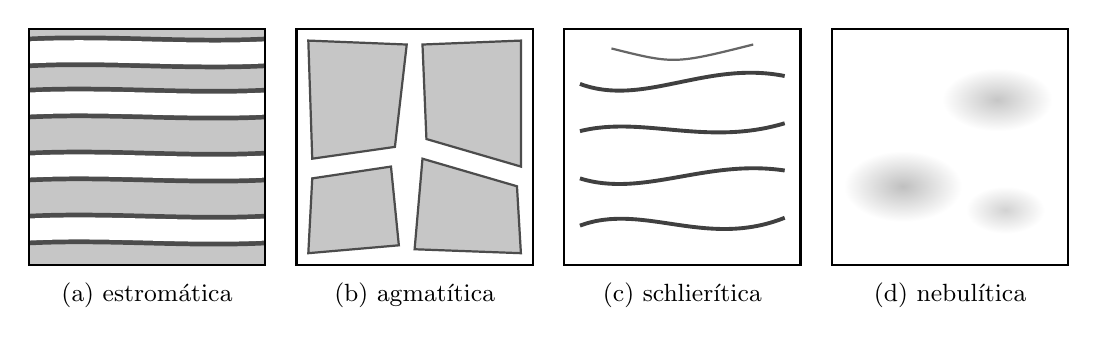
\begin{tikzpicture}[x=1cm, y=1cm]
% (a) stromatic
\begin{scope}
\fill[gray!45] (0,0) rectangle (3,3);
\foreach \y in {0.45, 1.25, 2.05, 2.7} {
  \fill[black!70] (0,\y-0.2) .. controls (1,\y-0.15) and (2,\y-0.25) .. (3,\y-0.2)
    -- (3,\y+0.2) .. controls (2,\y+0.15) and (1,\y+0.25) .. (0,\y+0.2) -- cycle;
  \fill[white] (0,\y-0.14) .. controls (1,\y-0.09) and (2,\y-0.19) .. (3,\y-0.14)
    -- (3,\y+0.14) .. controls (2,\y+0.09) and (1,\y+0.19) .. (0,\y+0.14) -- cycle;
}
\draw[thick] (0,0) rectangle (3,3);
\node[font=\small, anchor=north] at (1.5,-0.1) {(a) estromática};
\end{scope}
% (b) agmatitic
\begin{scope}[xshift=3.4cm]
\fill[white] (0,0) rectangle (3,3);
\fill[gray!45, draw=black!70, thick] (0.15,0.15) -- (1.3,0.25) -- (1.2,1.25) -- (0.2,1.1) -- cycle;
\fill[gray!45, draw=black!70, thick] (1.5,0.2) -- (2.85,0.15) -- (2.8,1.0) -- (1.6,1.35) -- cycle;
\fill[gray!45, draw=black!70, thick] (0.2,1.35) -- (1.25,1.5) -- (1.4,2.8) -- (0.15,2.85) -- cycle;
\fill[gray!45, draw=black!70, thick] (1.65,1.6) -- (2.85,1.25) -- (2.85,2.85) -- (1.6,2.8) -- cycle;
\draw[thick] (0,0) rectangle (3,3);
\node[font=\small, anchor=north] at (1.5,-0.1) {(b) agmatítica};
\end{scope}
% (c) schlieric
\begin{scope}[xshift=6.8cm]
\fill[white] (0,0) rectangle (3,3);
\foreach \y/\a in {0.5/0.3, 1.1/-0.25, 1.7/0.2, 2.3/-0.3} {
  \draw[black!75, line width=1.4pt] (0.2,\y) .. controls (1,\y+\a) and (1.8,\y-\a) .. (2.8,\y+0.1);
}
\draw[black!60, line width=0.8pt] (0.6,2.75) .. controls (1.4,2.55) .. (2.4,2.8);
\draw[thick] (0,0) rectangle (3,3);
\node[font=\small, anchor=north] at (1.5,-0.1) {(c) schlierítica};
\end{scope}
% (d) nebulitic
\begin{scope}[xshift=10.2cm]
\fill[white] (0,0) rectangle (3,3);
\shade[inner color=gray!50, outer color=white] (0.9,1.0) ellipse (0.75 and 0.45);
\shade[inner color=gray!45, outer color=white] (2.1,2.1) ellipse (0.7 and 0.4);
\shade[inner color=gray!35, outer color=white] (2.2,0.7) ellipse (0.5 and 0.3);
\draw[thick] (0,0) rectangle (3,3);
\node[font=\small, anchor=north] at (1.5,-0.1) {(d) nebulítica};
\end{scope}
\end{tikzpicture}
\par\smallskip{\small Cuatro estructuras de \omterm{def:b2:crustal-melting:migmatite}{migmatitas}, esquema (caras de afloramiento de cerca de un metro
de ancho). Blanco: \omterm{def:b2:crustal-melting:migmatite}{leucosoma}; negro: \omterm{def:b2:crustal-melting:migmatite}{melanosoma}; gris: mesosoma. (a) Estromática: capas de
\omterm{def:b2:crustal-melting:migmatite}{leucosoma}, cada una con un ribete oscuro, paralelas a la foliación, típica de las \omterm{def:b2:crustal-melting:migmatite}{metatexitas}.
(b) Agmatítica: una red de venas de \omterm{def:b2:crustal-melting:migmatite}{leucosoma} alrededor de bloques angulosos, con aspecto
brechoide. (c) Schlierítica: estrías de minerales oscuros dentro del \omterm{def:b2:crustal-melting:migmatite}{leucosoma}. (d) Nebulítica: fantasmas
difusos de la roca anterior en un huésped de aspecto ígneo; (c) y (d) son típicas de las
\omterm{def:b2:crustal-melting:migmatite}{diatexitas}.}
\end{omfigure}
% ledger: bgs99:migmatite, scmr:migmatite

\begin{omfigure}
\centering
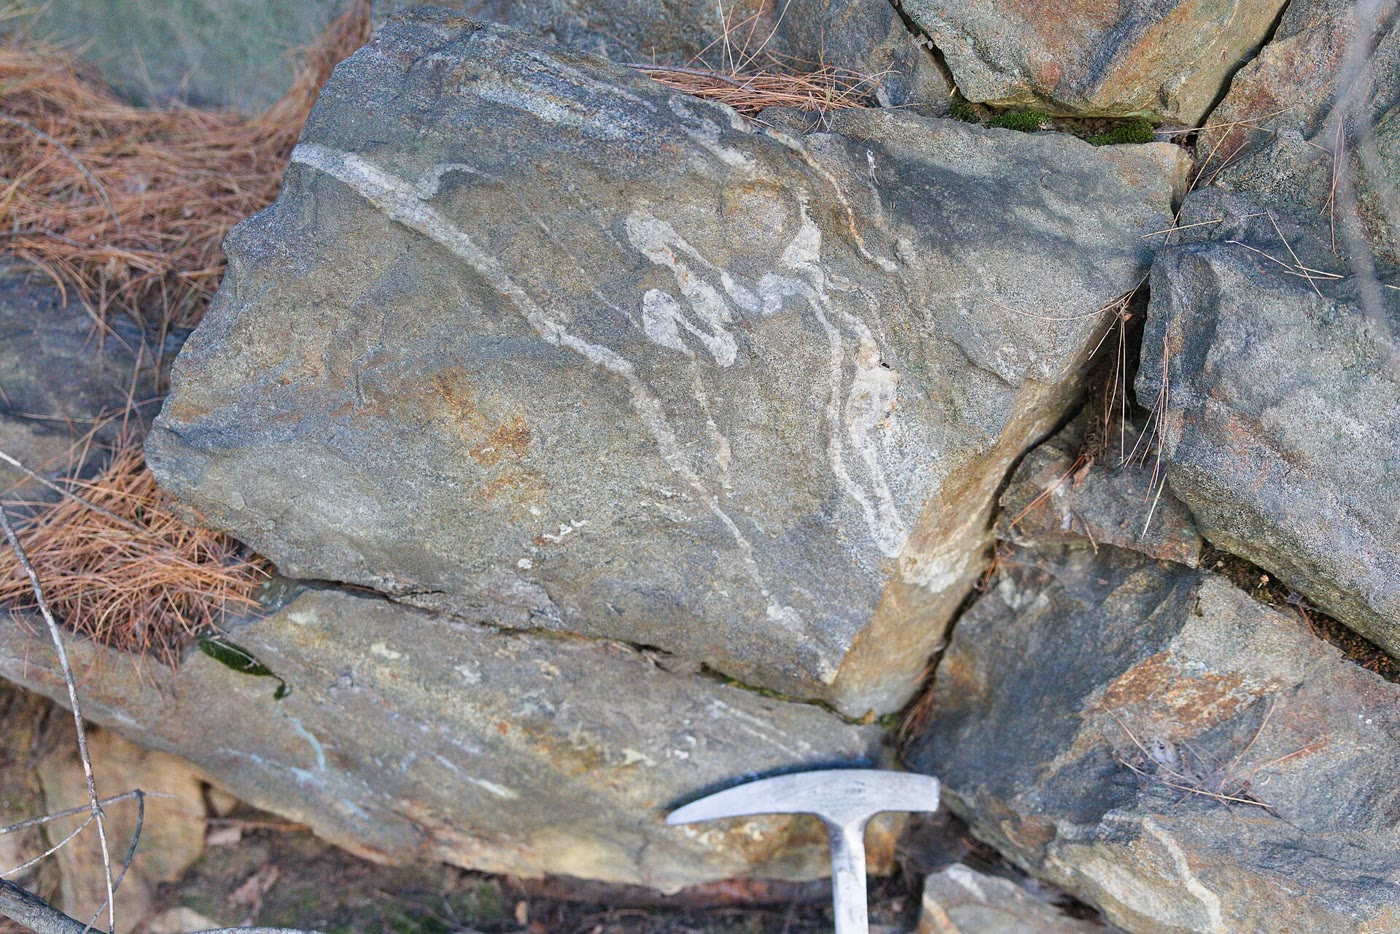
\includegraphics[width=0.62\linewidth]{images/book4/b2-12-migmatite.jpg}
\par\smallskip{\small Una \omterm{def:b2:crustal-melting:migmatite}{migmatita} en Nashua, New Hampshire: venas claras de \omterm{def:b2:crustal-melting:migmatite}{leucosoma}, plegadas
con el gneis gris que las contiene. El martillo del geólogo da la escala. Fotografía de Kevin M. Gill, CC BY 4.0.}
\end{omfigure}

\section{De la migmatita al plutón}\label{sec:b2:crustal-melting:segregation}

A la escala del grano, el primer fundido se sitúa a lo largo de los bordes de grano y en pequeñas bolsas,
sobre todo paralelas a la foliación. Por poco que sea, cambia la roca: en experimentos con
granito parcialmente fundido, la resistencia del agregado cae bruscamente entre el solidus
y una \omterm{def:b2:mantle-melting:fraction}{fracción de fundido} de \num{0.07}, a medida que se conectan los bordes de grano con fundido, y vuelve a caer,
unos cuatro órdenes de magnitud pero desde un valor ya bajo, cuando el armazón
cristalino se desmorona a fracciones de fundido mayores. La corteza parcialmente fundida es por tanto débil,
y la deformación se concentra en ella en cuanto empieza la fusión. La deformación, a su vez, impulsa el
fundido: drena de la matriz por bordes de grano conectados hacia \omterm{def:b2:crustal-melting:migmatite}{leucosomas} paralelos a
la foliación, y después fuera de la capa que funde por \omterm{def:b2:crustal-melting:migmatite}{leucosomas} que la cortan, y
estos confluyen en los \omterm{def:b2:magma-emplacement:bodies}{diques} del \cref{ch:b2:magma-emplacement}. La figura siguiente resume el
camino de la fuente al \omterm{def:b2:magma-emplacement:bodies}{plutón}.
% ledger: sawyer01:segregation, rh05:connectivity

\begin{omfigure}
\centering
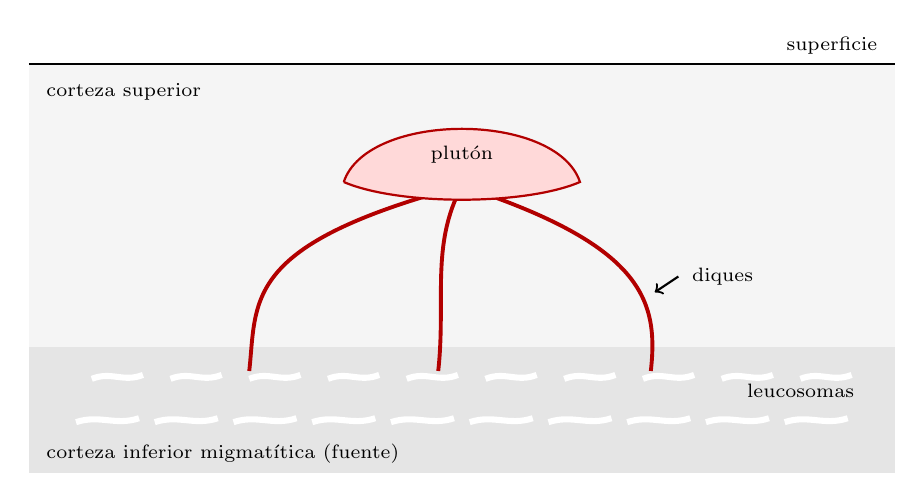
\begin{tikzpicture}[x=1cm, y=1cm]
\fill[gray!20] (0,0) rectangle (11,1.6);
\fill[gray!8] (0,1.6) rectangle (11,5.2);
\node[font=\scriptsize, anchor=west] at (0.1,0.25) {corteza inferior migmatítica (fuente)};
\foreach \x in {0.6,1.6,2.6,3.6,4.6,5.6,6.6,7.6,8.6,9.6} {
  \draw[white, line width=2.2pt] (\x,0.65) .. controls (\x+0.3,0.75) and (\x+0.5,0.6) .. (\x+0.8,0.7);
  \draw[white, line width=2.2pt] (\x+0.2,1.2) .. controls (\x+0.45,1.3) and (\x+0.6,1.15) .. (\x+0.85,1.25);
}
\foreach \x in {2.8, 5.2, 7.9} {
  \draw[red!70!black, line width=1.4pt] (\x,1.3) .. controls (\x+0.1,2.2) and (\x-0.1,2.9) .. (5.5,3.65);
}
\fill[pink!60, draw=red!70!black, thick] (4.0,3.7) .. controls (4.3,4.6) and (6.7,4.6) .. (7.0,3.7)
  .. controls (6.3,3.4) and (4.7,3.4) .. (4.0,3.7);
\node[font=\scriptsize] at (5.5,4.05) {plutón};
\node[font=\scriptsize, anchor=west] at (8.3,2.5) {diques};
\draw[->, thick] (8.25,2.5) -- (7.95,2.3);
\node[font=\scriptsize, anchor=west] at (0.1,4.85) {corteza superior};
\draw[thick] (0,5.2) -- (11,5.2);
\node[font=\scriptsize, anchor=south east] at (10.9,5.2) {superficie};
\node[font=\scriptsize, align=left, anchor=west] at (9.0,1.05) {leucosomas};
\end{tikzpicture}
\par\smallskip{\small De la \omterm{def:b2:crustal-melting:migmatite}{migmatita} al \omterm{def:b2:magma-emplacement:bodies}{plutón}, esquema sin escala: los \omterm{def:b2:crustal-melting:migmatite}{leucosomas}
(blanco) de la fuente parcialmente fundida confluyen en \omterm{def:b2:magma-emplacement:bodies}{diques} (rojo) que alimentan un \omterm{def:b2:magma-emplacement:bodies}{plutón} más arriba en
la corteza.}
\end{omfigure}

¿Cuánto tiempo permanece fundida la corteza? En el Himalaya, la \omterm{def:b2:crustal-melting:anatexis}{anatexia} generalizada empezó unos
30 millones de años después de la colisión de la India con Asia, y el circón y la monacita de las
rocas anatécticas dan edades de hace unos 25 a 15 millones de años; una sola muestra puede abarcar
la mayor parte de ese intervalo. La fusión de la corteza himalaya no fue un acontecimiento, sino un estado que
duró unos diez millones de años.
% ledger: weinberg16:himalaya

\section{Tipos de granito}\label{sec:b2:crustal-melting:types}

Un granito recuerda su fuente en su química, ante todo en cuánto aluminio contiene
en comparación con el que pueden admitir sus feldespatos.

\begin{definition}[Índice de saturación en aluminio]\label{def:b2:crustal-melting:asi}
El \emph{índice de saturación en aluminio}\index{indice de saturación en aluminio@índice de saturación en aluminio} de una roca es la
razón molar
\[\mathrm{A/CNK} = \frac{n(\ce{Al2O3})}{n(\ce{CaO}) + n(\ce{Na2O}) + n(\ce{K2O})},\]
y su compañero es $\mathrm{A/NK} = n(\ce{Al2O3})/[n(\ce{Na2O}) + n(\ce{K2O})]$. Una roca
es \emph{peraluminosa}\index{peraluminosa} si $\mathrm{A/CNK} > 1$,
\emph{metaluminosa}\index{metaluminosa} si $\mathrm{A/CNK} < 1 < \mathrm{A/NK}$, y
\emph{peralcalina}\index{peralcalina} si $\mathrm{A/NK} < 1$.
\end{definition}
% ledger: moyen17:aluminosity, frost01:asi

\begin{proposition}[Lo que mide el índice]\label{prop:b2:crustal-melting:feldspar}
Una roca cuyo calcio, sodio y potasio están todos en feldespatos, y cuyo aluminio está
todo en feldespatos, tiene $\mathrm{A/CNK} = 1$. Por tanto, a una roca \omterm{def:b2:crustal-melting:asi}{peraluminosa} le sobra aluminio
después de sus feldespatos, alojado en minerales alumínicos (moscovita, granate, cordierita,
aluminosilicato); a una roca \omterm{def:b2:crustal-melting:asi}{metaluminosa} le sobra calcio, alojado en silicatos cálcicos
(hornblenda, clinopiroxeno, titanita); y a una roca \omterm{def:b2:crustal-melting:asi}{peralcalina} le sobran sodio y potasio,
alojados en minerales sin aluminio suficiente para formar feldespato (piroxeno sódico y
anfíbol sódico).
\end{proposition}

\begin{proof}
En forma de óxidos, la fórmula del feldespato potásico es \ce{K2O.Al2O3.6SiO2}, la de la albita, \ce{Na2O.Al2O3.6SiO2}, y
la de la anortita, \ce{CaO.Al2O3.2SiO2}: cada una tiene exactamente un \ce{Al2O3} por cada
\ce{K2O}, \ce{Na2O} o \ce{CaO}. Cualquier mezcla de los tres tiene por tanto $n(\ce{Al2O3}) =
n(\ce{CaO}) + n(\ce{Na2O}) + n(\ce{K2O})$, es decir, $\mathrm{A/CNK} = 1$. Si
$\mathrm{A/CNK} > 1$, el aluminio supera lo que los álcalis y el calcio pueden fijar en
feldespato, y el exceso tiene que alojarse en otros minerales. Si $\mathrm{A/CNK} < 1$ pero
$\mathrm{A/NK} > 1$, hay aluminio suficiente para todo el sodio y el potasio en forma de
feldespato, pero no para todo el calcio, que va a minerales que necesitan menos aluminio
por calcio que la anortita. Si $\mathrm{A/NK} < 1$, ni siquiera los álcalis pueden estar todos en
feldespato.
\end{proof}

Moyen y colaboradores hallaron que la aluminosidad es el indicador más útil para distinguir granitos
de fuentes distintas; Frost y colaboradores usan el mismo índice, con una pequeña
corrección por el fósforo, como uno de los tres ejes de su clasificación de las rocas
graníticas.
% ledger: moyen17:aluminosity, frost01:asi

\begin{omfigure}
\centering
\begin{tikzpicture}
\begin{axis}[omrecord, width=0.72\linewidth, height=7cm,
  xmin=0.4, xmax=1.5, ymin=0.4, ymax=3.5, xlabel={A/CNK (molar)}, ylabel={A/NK (molar)},
  tick label style={font=\scriptsize}, label style={font=\small}]
\addplot[fill=gray!15, draw=none] coordinates {(0.4,0.4) (1.5,1.5) (1.5,0.4) (0.4,0.4)};
\addplot[thick, black!70] coordinates {(1,0.4) (1,3.5)};
\addplot[thick, black!70] coordinates {(0.4,1) (1.5,1)};
\node[font=\scriptsize, anchor=north east] at (axis cs:1.48,3.45) {peraluminosa};
\node[font=\scriptsize, anchor=west] at (axis cs:0.62,2.6) {metaluminosa};
\node[font=\scriptsize, anchor=south west] at (axis cs:0.42,0.45) {peralcalina};
\addplot[only marks, mark=*, mark size=2pt, blue!70!black, nodes near coords,
  point meta=explicit symbolic, every node near coord/.style={font=\scriptsize, anchor=west}]
  coordinates {(0.539,3.196)[BHVO-2] (0.877,1.694)[AGV-2] (0.993,1.135)[SRM 278]};
\addplot[only marks, mark=square*, mark size=2pt, red!70!black]
  coordinates {(1.261,1.377) (0.809,0.844)};
\node[font=\scriptsize, red!70!black, anchor=south] at (axis cs:1.261,1.45) {fundido de tipo S};
\node[font=\scriptsize, red!70!black, anchor=north] at (axis cs:0.809,0.79) {granito peralcalino};
\end{axis}
\end{tikzpicture}
\par\smallskip{\small Diagrama de Shand. Círculos azules: tres materiales de referencia, un basalto
hawaiano (BHVO-2), una andesita (AGV-2) y una obsidiana de composición granítica (SRM 278),
calculados a partir de sus contenidos de óxidos publicados. Cuadrados rojos: dos granitos inventados que se usan en
este capítulo. El triángulo gris es inalcanzable, ya que A/CNK nunca supera A/NK.}
\end{omfigure}
% ledger: usgs:bhvo2-major, usgs:agv2-major, nist278:majors

La química sigue a la fuente. En 1974, Chappell y White observaron que, salvo las rocas
más félsicas, los granitos del Cinturón Plegado de Lachlan se reparten en dos grupos bien distintos,
y los interpretaron como fundidos de dos clases de roca fuente: rocas ígneas más antiguas y rocas sedimentarias. La hidrólisis de los feldespatos, vista en el volumen de primer
año, se lleva en disolución el sodio y el calcio y retiene el aluminio en las arcillas: los lodos formados
por esas arcillas son ricos en aluminio, y también lo son sus fundidos.
% ledger: cw01:is-types

\begin{definition}[Tipología de los granitos]\label{def:b2:crustal-melting:types}
Un \emph{granito de tipo I}\index{granito de tipo I} es un granito cuya fuente fue sobre todo una
roca ígnea más antigua; un \emph{granito de tipo S}\index{granito de tipo S}, uno cuya fuente fue
sobre todo una roca sedimentaria (metasedimentaria); y un granito de tipo M, uno derivado
del manto. Un \emph{granito de tipo A}\index{granito de tipo A} se define por su química y su
contexto más que por su fuente: ferroso y potásico, muy enriquecido en \omterm{def:b2:elements-in-the-earth:partition}{elementos incompatibles},
y emplazado en contextos estables de intraplaca, de trasarco o poscolisionales.
\end{definition}
% ledger: johansson23:a-type, cw01:is-types

Los \omterm{def:b2:crustal-melting:types}{granitos de tipo S} son peraluminosos, con dos micas o con cordierita; los granitoides de tipo A
son en su mayoría metaluminosos, algunos peraluminosos. Un solo análisis puede engañar, sin embargo: toda
serie de granitoides termina cerca de la composición del mínimo granítico, leucocrática y ligeramente
\omterm{def:b2:crustal-melting:asi}{peraluminosa}, de modo que una muestra \omterm{def:b2:crustal-melting:asi}{peraluminosa} no prueba que se fundiera corteza. Lo que distingue
unas series de otras es la forma de su tendencia en el diagrama de Shand: una serie de arco llega al
mínimo por una alineación empinada desde A/NK alto y A/CNK bajo; una serie de tipo S pobre en calcio,
por una alineación con A/NK próximo a A/CNK. No se ha llegado a un consenso sobre la fuente de los
\omterm{def:b2:magma-emplacement:magma}{magmas} de tipo A: un modelo los forma a partir de basalto subplacado, evolucionado por cristalización,
\omterm{def:b2:mantle-melting:melting}{fusión parcial} y asimilación de corteza.
% ledger: moyen17:trends, frost01:asi, johansson23:a-type

\begin{definition}[Leucogranito]\label{def:b2:crustal-melting:leucogranite}
Un \emph{leucogranito}\index{leucogranito} es un granito de color claro, casi libre de
minerales oscuros; los leucogranitos peraluminosos de los cinturones de colisión llevan moscovita, sola o
con biotita.
\end{definition}
% ledger: moyen17:aluminosity, pdh98:himalaya

Los \omterm{def:b2:crustal-melting:leucogranite}{leucogranitos} peraluminosos con moscovita de los cinturones de colisión tienen composiciones próximas
a las de los líquidos de la fusión en presencia de agua o de la \omterm{def:b2:crustal-melting:reactions}{fusión por deshidratación} de la moscovita, a temperaturas cercanas a
\qty{700}{\celsius}, a las que el circón y la monacita de la fuente pueden sobrevivir y ser arrastrados
al fundido como xenocristales; los granitos peraluminosos con cordierita proceden de la
descomposición, más caliente, de la biotita, a 800--\qty{850}{\celsius}. Los \omterm{def:b2:crustal-melting:leucogranite}{leucogranitos} del Himalaya,
con su fuerte firma isotópica cortical, pertenecen a esta familia
(\cref{ch:b2:himalaya-andes}).
% ledger: moyen17:aluminosity, weinberg16:himalaya

\begin{omfigure}
\centering
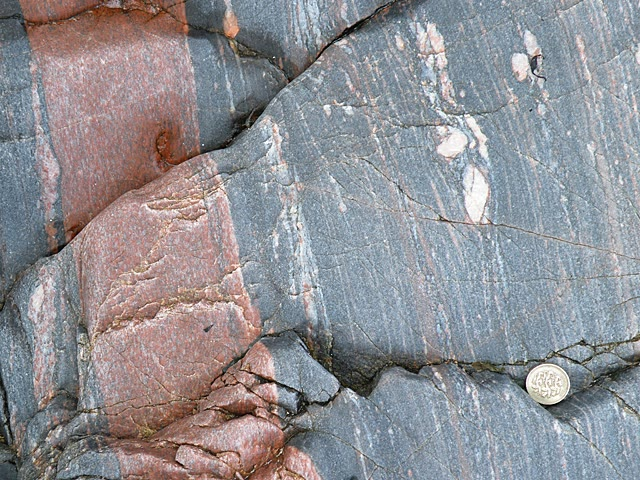
\includegraphics[width=0.5\linewidth]{images/book4/b2-12-leucogranite-vein.jpg}
\par\smallskip{\small Una vena rosada de \omterm{def:b2:crustal-melting:leucogranite}{leucogranito} que corta un gneis gris bandeado; la moneda da
la escala. Fotografía de Anne Burgess (Geograph), CC BY-SA 2.0.}
\end{omfigure}

\section{Los granitos y el crecimiento de los continentes}\label{sec:b2:crustal-melting:time}

Dos clases de lugares producen la mayor parte del granito. Sobre las zonas de subducción, la corteza de arco se forma por
diferenciación de fundidos máficos procedentes del manto, y el calor disponible es solo el que aportan esos
fundidos. Tras una colisión, la corteza engrosada es un sistema muy caliente: funde a gran
escala, a baja temperatura donde el agua o la moscovita lo permiten y a temperatura más alta
por descomposición de la biotita, y esos granitos de origen cortical reciclan corteza que
ya existía. Los fundidos del manto también llegan allí a la corteza, en cantidades lo bastante grandes, sostienen Moyen y
colaboradores, como para que los cinturones tardiorogénicos contribuyan de forma importante al crecimiento de la
corteza. Que un granito añada material a los continentes o solo los retrabaje es, pues, una cuestión de
su fuente, a la que responden sus isótopos (\cref{ch:b2:isotope-geochemistry}); los granitos de
la Tierra primitiva, muy distintos de estos, son el tema del
\cref{ch:b2:precambrian-earth}.
% ledger: moyen17:settings

\section{Ejercicios}\label{sec:b2:crustal-melting:exercises}

Masas molares (\unit{\gram\per\mole}): \ce{Al2O3} 101.96, \ce{CaO} 56.08, \ce{Na2O} 61.98,
\ce{K2O} 94.20, \ce{H2O} 18.02; masas atómicas: H 1.008, O 16.00, Na 22.99, Mg 24.31,
Al 26.98, Si 28.09, K 39.10, Ca 40.08. Tómese $g = \qty{9.81}{\metre\per\second\squared}$.

\begin{exercise}[$\star$]\label{exo:b2:crustal-melting:1}
El material de referencia andesítico AGV-2 contiene, en \unit{\gram} por \qty{100}{\gram},
\ce{Al2O3} 17.03, \ce{CaO} 5.15, \ce{Na2O} 4.204 y \ce{K2O} 2.898.
(a) Calcúlense su A/CNK y su A/NK. (b) Clasifíquese, y nómbrese un mineral que debería alojar su
exceso de calcio.
\end{exercise}
% ledger: usgs:agv2-major

\begin{exercise}[$\star$]\label{exo:b2:crustal-melting:2}
Tres granitos contienen, además de cuarzo y feldespatos: (a) moscovita, biotita y granate;
(b) hornblenda, biotita y titanita; (c) egirina, un piroxeno de sodio y hierro
\ce{NaFeSi2O6}, y un anfíbol sódico. Clasifíquese cada uno según su saturación en aluminio, y dígase
cuál podría ser un \omterm{def:b2:crustal-melting:types}{granito de tipo S}.
\end{exercise}

\begin{exercise}[$\star$]\label{exo:b2:crustal-melting:3}
Una corteza de densidad \qty{2800}{\kilogram\per\cubic\metre} tiene una geoterma lineal
$T = \qty{10}{\celsius} + (\qty{20}{\celsius\per\kilo\metre})\,z$. Entre 2 y
\qty{10}{kbar}, aproxímese el solidus del granito húmedo por la recta que pasa por
(\qty{680}{\celsius}, \qty{2}{kbar}) y (\qty{620}{\celsius}, \qty{10}{kbar}). ¿A qué
profundidad, temperatura y presión la corta la geoterma?
\end{exercise}
% ledger: sw81:wet-solidus

\begin{exercise}[$\star$]\label{exo:b2:crustal-melting:4}
Un gneis gris de biotita lleva capas blancas de cuarzo y feldespato de un centímetro de espesor, paralelas
a su foliación, cada una bordeada por un fino ribete negro de biotita; entre las capas el
gneis parece normal. (a) Nómbrense las capas blancas, los ribetes negros y el gneis normal.
(b) ¿Es la roca una \omterm{def:b2:crustal-melting:migmatite}{metatexita} o una \omterm{def:b2:crustal-melting:migmatite}{diatexita}, y cuál es su estructura? (c) A unos cientos de
metros, el bandeado ha desaparecido: una roca estriada, de aspecto granítico, conserva tenues fantasmas de
gneis. ¿Qué ha cambiado?
\end{exercise}
% ledger: scmr:migmatite, bgs99:migmatite

\begin{exercise}[$\star\star$]\label{exo:b2:crustal-melting:5}
Tómese la biotita como flogopita, \ce{KMg3AlSi3O10(OH)2}. (a) Calcúlense su masa molar y la
fracción másica de agua que libera (sus dos grupos hidroxilo dan un \ce{H2O}).
(b) Un gneis con un \qty{25}{\percent} de biotita en masa funde por \omterm{def:b2:crustal-melting:reactions}{fusión por deshidratación} de la biotita
dando un fundido con un \qty{4.0}{\percent} de agua. Con ayuda de la
\cref{prop:b2:crustal-melting:water}, hállese la \omterm{def:b2:mantle-melting:fraction}{fracción de fundido}, y compárese con las
fracciones halladas en experimentos de \omterm{def:b2:crustal-melting:reactions}{fusión por deshidratación} de la biotita.
\end{exercise}
% ledger: bk99:migmatites

\begin{exercise}[$\star\star$]\label{exo:b2:crustal-melting:6}
Cien gramos de granito contienen \qty{30}{\gram} de feldespato potásico \ce{KAlSi3O8},
\qty{35}{\gram} de albita \ce{NaAlSi3O8}, \qty{5}{\gram} de anortita \ce{CaAl2Si2O8},
\qty{25}{\gram} de cuarzo y \qty{5}{\gram} de moscovita \ce{KAl3Si3O10(OH)2}.
(a) Calcúlense las masas molares de los cuatro minerales alumínicos. (b) Calcúlense las cantidades de
\ce{Al2O3}, \ce{CaO}, \ce{Na2O} y \ce{K2O} en la roca, y su A/CNK. (c) ¿Qué
mineral hace \omterm{def:b2:crustal-melting:asi}{peraluminosa} la roca?
\end{exercise}

\begin{exercise}[$\star\star$]\label{exo:b2:crustal-melting:7}
Un sill basáltico intruido a \qty{1200}{\celsius} cristaliza por completo y se enfría hasta
\qty{850}{\celsius}, liberando un calor latente de \qty{900}{\mega\joule\per\cubic\metre}.
La corteza que lo rodea, a \qty{650}{\celsius}, se calienta hasta \qty{850}{\celsius} y
se funde en un \qty{20}{\percent}, con el mismo calor latente por unidad de volumen de fundido. Ambas
rocas tienen una capacidad calorífica de \qty{2.5}{\mega\joule\per\cubic\metre\per\kelvin}. Con ayuda de la
\cref{prop:b2:crustal-melting:heat}, ¿cuántos metros cúbicos de corteza puede tratar así un metro cúbico
de basalto? ¿Qué deja de lado el resultado?
\end{exercise}
% ledger: delaney86b4:properties

\begin{exercise}[$\star\star$]\label{exo:b2:crustal-melting:8}
El material de referencia de obsidiana SRM 278 está certificado en \ce{Al2O3}
$14.15 \pm 0.15$, \ce{CaO} 0.983, \ce{Na2O} 4.84 y \ce{K2O} 4.16 (\unit{\percent} en
masa). (a) Calcúlense su A/CNK y su A/NK, y clasifíquese. (b) Recalcúlese A/CNK con los dos
extremos de la incertidumbre de \ce{Al2O3}. ¿Es robusta la clasificación?
\end{exercise}
% ledger: nist278:majors

\begin{exercise}[$\star\star$]\label{exo:b2:crustal-melting:9}
A \qty{800}{\celsius}, un fundido haplogranítico saturado en agua contiene un \qty{7.45}{\percent}
de agua a \qty{3}{kbar}, 8.94 a \qty{4}{kbar}, 9.97 a \qty{5}{kbar} y 13.82 a
\qty{8}{kbar}. (a) Ajústese una recta a estos cuatro puntos por mínimos cuadrados y compárese
su pendiente con el \qty{1.27}{\percent} por kilobar que dan los experimentadores.
(b) Predígase el contenido de saturación a \qty{6}{kbar}. (c) ¿Cuál es la masa mínima de fundido
que puede transportar \qty{10}{\gram} de agua a \qty{6}{kbar}? (d) ¿Por qué no debe
usarse la recta a \qty{15}{kbar}?
\end{exercise}
% ledger: holtz95:solubility

\begin{exercise}[$\star\star\star$]\label{exo:b2:crustal-melting:10}
Aproxímese el solidus de \omterm{def:b2:crustal-melting:reactions}{fusión por deshidratación} de un esquisto con moscovita por la recta que pasa
por (\qty{750}{\celsius}, \qty{6}{kbar}) y (\qty{800}{\celsius}, \qty{10}{kbar}),
los extremos de los intervalos experimentales. Un esquisto a \qty{770}{\celsius} sube desde
\qty{10}{kbar} sin ganar ni perder calor. (a) ¿A qué presión alcanza el
solidus? (b) Más allá, su temperatura sigue el solidus hacia abajo, y el calor de la fusión procede
de su propio enfriamiento. Con una capacidad calorífica de \qty{2.5}{\mega\joule\per\cubic\metre\per\kelvin}
y un calor latente de \qty{900}{\mega\joule\per\cubic\metre}, ¿qué \omterm{def:b2:mantle-melting:fraction}{fracción de fundido} en volumen
se ha formado cuando llega a \qty{6}{kbar}? (c) Compárese con las condiciones propuestas para los
\omterm{def:b2:crustal-melting:leucogranite}{leucogranitos} del Himalaya.
\end{exercise}
% ledger: pdh98:himalaya, delaney86b4:properties

\begin{exercise}[$\star\star\star$]\label{exo:b2:crustal-melting:11}
El calor se difunde sobre una distancia $\ell$ en un tiempo del orden de $\ell^2/\kappa$. Con
$\kappa = \qty{1e-6}{\square\metre\per\second}$, estímese el tiempo que tarda el calor de un
sill de \qty{2}{km} de espesor, y de una capa subplacada de \qty{10}{km} de espesor, en extenderse sobre su
propio espesor. Compárese con los diez millones de años de \omterm{def:b2:crustal-melting:anatexis}{anatexia} himalaya: ¿puede un único
episodio de subplacado explicarla?
\end{exercise}
% ledger: delaney86b4:properties, weinberg16:himalaya

\begin{exercise}[$\star\star\star$]\label{exo:b2:crustal-melting:12}
Se analiza una \omterm{def:b2:crustal-melting:migmatite}{migmatita} estromática: \omterm{def:b2:crustal-melting:migmatite}{leucosoma} \ce{K2O} \qty{5.0}{\percent}, \ce{MgO}
\qty{0.20}{\percent}; \omterm{def:b2:crustal-melting:migmatite}{melanosoma} \ce{K2O} \qty{2.0}{\percent}, \ce{MgO}
\qty{4.0}{\percent}; mesosoma, tomado como el \omterm{def:b2:metamorphic-facies:metamorphism}{protolito} no fundido, \ce{K2O}
\qty{2.75}{\percent}, \ce{MgO} \qty{3.05}{\percent} (todo en masa). (a) Si el
neosoma se formó a partir del \omterm{def:b2:metamorphic-facies:metamorphism}{protolito} sin ganancia ni pérdida, ¿qué fracción másica de él es
\omterm{def:b2:crustal-melting:migmatite}{leucosoma}? (b) Compruébese la respuesta con el \ce{MgO}. (c) En el afloramiento el \omterm{def:b2:crustal-melting:migmatite}{leucosoma} solo forma un
\qty{10}{\percent} del neosoma en masa. ¿Cuántos gramos de fundido se fueron por cada
\qty{100}{\gram} de roca original?
\end{exercise}

\begin{problem}[{Problema de fin de semana --- un plutón de mica fundida}]\label{pb:b2:crustal-melting:1}
Un esquisto formado por un \qty{20}{\percent} de moscovita, un \qty{15}{\percent} de biotita, un
\qty{30}{\percent} de cuarzo, un \qty{30}{\percent} de plagioclasa y un \qty{5}{\percent} de otros
minerales (en masa; una roca inventada) se encuentra en la base de una corteza duplicada por apilamiento, la
situación modelizada en el \cref{ch:b2:pt-paths}. Puede fundirse y alimentar un \omterm{def:b2:magma-emplacement:bodies}{plutón} granítico. Datos:
las masas atómicas y molares del encabezado de los ejercicios; el solidus del granito húmedo pasa
por (\qty{680}{\celsius}, \qty{2}{kbar}), (\qty{620}{\celsius}, \qty{10}{kbar}),
(\qty{605}{\celsius}, \qty{15.3}{kbar}) y (\qty{670}{\celsius}, \qty{27}{kbar}); el
contenido de saturación en agua de un fundido granítico a \qty{800}{\celsius} es del \qty{9.97}{\percent} a
\qty{5}{kbar} y del \qty{13.82}{\percent} a \qty{8}{kbar}. La base de la corteza engrosada del modelo evoluciona así:

\smallskip
\begin{center}\small
\begin{tabular}{l|ccccccccccc}
$t$ (\unit{Myr}) & 0 & 10 & 20 & 30 & 40 & 50 & 60 & 70 & 80 & 90 & 100\\ \hline
$T$ (\unit{\celsius}) & 595 & 656 & 734 & 795 & 845 & 885 & 909 & 914 & 900 & 867 & 814\\
$P$ (\unit{kbar}) & 19.2 & 19.2 & 19.2 & 19.2 & 17.9 & 16.5 & 15.1 & 13.7 & 12.4 & 11.0 & 9.6
\end{tabular}
\end{center}
\smallskip

\noindent\textbf{Parte I --- El agua de la mica.}
\begin{enumerate}
\item Calcúlese la masa molar de la moscovita \ce{KAl3Si3O10(OH)2}.
\item Sus dos grupos hidroxilo dan un \ce{H2O}. ¿Qué fracción másica del mineral se
libera como agua?
\item ¿Cuánta agua libera la moscovita de un kilogramo de esquisto?
\item Interpolando linealmente, ¿cuál es el contenido de agua de saturación del fundido a
\qty{7}{kbar}? ¿Cuál es entonces la fracción mínima de fundido que puede formar el agua de la moscovita?
\item El fundido de la \omterm{def:b2:crustal-melting:reactions}{fusión por deshidratación} está lejos de la saturación; tómese su contenido de agua como
\qty{6.0}{\percent}. ¿Qué \omterm{def:b2:mantle-melting:fraction}{fracción de fundido} forma la moscovita?
\item En experimentos con una \omterm{def:b2:metamorphic-facies:protoliths}{metapelita} de dos micas a \qty{10}{kbar}, la reacción de la moscovita
dio solo de un 1 a un \qty{2}{\percent} de fundido. Dense dos razones por las que una roca real puede producir menos
fundido que lo obtenido en la pregunta~5.
\end{enumerate}

\noindent\textbf{Parte II --- El calentamiento de la fuente.}
\begin{enumerate}[resume]
\item En el \cref{ch:b2:pt-paths}, la roca que queda en la corteza media alcanza un pico de \qty{593}{\celsius}
y \qty{7.8}{kbar}. ¿Cuál es el solidus húmedo a \qty{7.8}{kbar}? ¿Puede fundir esa roca, incluso
con agua libre?
\item Interpolando entre 15.3 y \qty{27}{kbar}, hállese el solidus húmedo a la presión
de la base justo después del apilamiento. ¿Está la base por encima de él en $t = 0$? ¿Y en $t = \qty{10}{Myr}$?
\item ¿Qué limita la fusión de la base en $t = \qty{10}{Myr}$, y por qué se detiene
pronto?
\item ¿Cuándo supera la base los \qty{800}{\celsius}, el extremo superior del intervalo de la
moscovita?
\item El intervalo del anfíbol abarca de 875 a \qty{925}{\celsius} a 10--\qty{12.5}{kbar}.
¿Cuándo entra la base en ese intervalo de presiones, y a qué temperatura?
\item ¿Cuándo alcanza la base los \qty{10}{kbar}, el techo del intervalo de presiones de los
experimentos con moscovita, y qué temperatura tiene entonces? ¿Qué minerales hidratados del esquisto pueden
existir todavía?
\end{enumerate}

\noindent\textbf{Parte III --- ¿Qué fundido?}
El fundido, una vez cristalizado, da un \omterm{def:b2:crustal-melting:leucogranite}{leucogranito} (análisis inventado) con, en
\unit{\percent} en masa, \ce{Al2O3} 15.0, \ce{CaO} 0.55, \ce{Na2O} 3.4 y \ce{K2O} 4.9.
\begin{enumerate}[resume]
\item Calcúlense las cantidades de los cuatro óxidos en \qty{100}{\gram} de la roca.
\item Calcúlese su A/CNK.
\item Calcúlese su A/NK y clasifíquese el \omterm{def:b2:crustal-melting:leucogranite}{leucogranito}.
\item ¿Es un \omterm{def:b2:crustal-melting:types}{granito de tipo I} o de tipo S? Nómbrense dos minerales que deberían alojar su exceso
de aluminio.
\item ¿Cuántos moles de \ce{Al2O3} por \qty{100}{\gram} sobran después de los
feldespatos? Si todo fuera a la moscovita, que contiene un \ce{Al2O3} más por unidad
de fórmula que el feldespato potásico, ¿cuántos gramos de moscovita contendrían
\qty{100}{\gram} de granito?
\item La obsidiana SRM 278 tiene A/CNK $= 0.993$. ¿Podrían el \omterm{def:b2:crustal-melting:leucogranite}{leucogranito} y la obsidiana
proceder de la misma clase de fuente?
\end{enumerate}

\noindent\textbf{Parte IV --- ¿Cuánta corteza?}
Un \omterm{def:b2:magma-emplacement:bodies}{plutón} inventado de este \omterm{def:b2:crustal-melting:leucogranite}{leucogranito} tiene un volumen de \qty{1000}{\cubic\kilo\metre}.
Tómense \qty{2650}{\kilogram\per\cubic\metre} para el granito y
\qty{2800}{\kilogram\per\cubic\metre} para el esquisto; supóngase que un \qty{70}{\percent} del
fundido abandona su fuente y que toda el agua del fundido escapa al cristalizar.
\begin{enumerate}[resume]
\item ¿Cuál es la masa del \omterm{def:b2:magma-emplacement:bodies}{plutón}?
\item ¿Qué masa de fundido (con su \qty{6.0}{\percent} de agua) hizo falta?
\item Con la \omterm{def:b2:mantle-melting:fraction}{fracción de fundido} de la pregunta~5, ¿qué masa de esquisto tuvo que fundirse?
\item ¿Qué volumen de esquisto es ese?
\item Si la fuente era una capa de \qty{5}{km} de espesor, ¿sobre qué superficie se fundió?
\item Con la fracción mínima de fundido de la pregunta~4, ¿cuánto mayor sería la
fuente? Dese el volumen de corteza fuente fundida para formar el \omterm{def:b2:magma-emplacement:bodies}{plutón}, en
\unit{\cubic\kilo\metre}, a partir de la pregunta~22.
\end{enumerate}
\end{problem}
